
\documentclass[10pt]{article}
\usepackage{graphicx}
\usepackage{blindtext}
\usepackage{tree-dvips}
\usepackage{float}
\usepackage[nottoc]{tocbibind}
\usepackage{url}
\usepackage[hidelinks]{hyperref}
\usepackage[T1]{fontenc}
\hypersetup{
    colorlinks,
    citecolor=black,
    filecolor=black,
    linkcolor=black,
    urlcolor=black
}
\graphicspath{ {./Misc/} }
\begin{document}
\title{Social And Visual Marketing: Privacy}
\author{Saleh Elhadidy}
\maketitle
\newpage
\tableofcontents
\newpage
\section{Background}
\subsection{Machine Learning}
Currently one of the trending fields in Artifical Intelligence (AI). Machine learning is generally considered as a subset of AI since it has the ability to learn and act without being
excplicitly programmed. It works by generalizing certian patterns instead of storing the input data and trying to match it exactly\cite{Intro}. For example, building an application to recognize
cats and dogs using Machine Learning can be done by showing the application pictures of different cats and dogs and having the application remember "features" of the cats and dogs to be
able to classify them later on. On the other hand using a traditional apprach storing all available pictures of cats and dogs and then later matching pictures exactly with the stored pictures.
\subsection{Homomorphic Encryption}
After investigating what the latest advances in academic research regarding encryption had reached we came to the conclusion that Homomprhic encryption was the most suitable encryption scheme to use,
To give a brief introduction, Homomorphic encryption is a form of encryption that allows computation on ciphertexts, generating an encrypted result which, when decrypted, matches the result of the operations as if they had been performed on the plaintext.
This makes homomorphic encryption the best candidate in Machine Learning as a service and cloud computing applications.\\
In this study we have compiled the three best implementations of Homomorphic Encryption to the best of our knowledge
\subsubsection{PALISADE}
Palisade is an open source highly protable cryptography library that supports Homomorphic Encryption. The project was previously funded by the NSA and is developed and maintained by the cryptography
team at New Jersey Institute of Technology. At the time of writing this PALISADE doesn't support floating point operations as it doesn't support CKKS Homomorphic Encryption scheme
\subsubsection{HELib}
Homomorphic Encryption Library is the second open source library that we looked at, HELib is developed and maintained by Shai Halevi and Victor Shoup.
HELib supports both BGV and CKKS encryption schemes which allows for operations on floating point numbers.
The downside to using HELib is that it less maintained due to the low number of contributors.
\subsubsection{Microsoft SEAL}
SEAL is a library that is built by Microsoft’s Cryptography team at Microsoft Research\cite{SEAL}.
The advantage of SEAL is that it supports both BGV/BFV and CKKS as well being the most documented library of the three.
It also has no dependencies making it modular in addition to having a CMAKE file which is used to build for various environments making it easy to compile and run.\\

It was also demonstrated that SEAL can be used in privacy preserving Machine Learning where the user data was encrypted on-device and the cloud server operated on the encrypted data providing
full user annonymity. The demonstration used the MNIST optical character dataset where an accuracy of 99\% was achieved\cite{gilad2016cryptonets}
\section{Methodology And Implementation}

Our goal was to explore whether privacy preserving ML would yield results similar to ML techniques without any privacy constraints and whether data obfuscation techniques can be enough to protect user data or can obfuscated data be de-anonymized.
We had a couple of approaches in mind for the privacy preserving ML, the first was using known data anonymization techniques such as on device face bluring/automated metadata deleteion and 
finally the last approach which was more complicated was trying to use homomorphic encryption and passing encrypted data the the Machine Learning Model.
However to be able to test these techniques we had to first collect enough data to be able to analyze our results and tweak our machine learning models so we decided to run an experiment on students in the GUC which involved developing a system that would gather data from user-submitted images and provide brand recognition and personal recommendation based on the each user’s preferences.
We also disclosed that all data gathered will be anonymized and will be deleted at the end of the bachelor thesis.
As for the  data obfuscation and data de-anonymization we had to generate our own dataset and classifier as this area hasn't been explored in recent research.
\subsection{Privacy Preserving Machine Learning}
\subsubsection{System Design}
The system consisted of a cross-platform Instagram-like mobile application that was developed using Facebook's React-Native, As for the backend we opted for Google's Firebase as the backend provider as it provided multiple advantages over other competitors namely, seamless authentication,
realtime database that was shared across all platforms, access to built-in on device and cloud basic Machine Learning models such as facial recognition and object recognition, the ability to deploy custom Machine Learning (ML) models within the same server and lastly, the ability to scale easily.


A social application was chosen to get the most user interaction which in turn would mean more user data to pass of the ML model.
The experiment was run as follows, whenever a user signed up the application would prompt an initial questionnaire to get a basic idea about the user’s preferences which would later be used in personalization,
the user would then  get a daily notification to post one or more images while on university campus for a given period of time.
Users also had the ability to “like” any image posted by any other user to further their preferences. 
\begin{figure}[H]
\centering
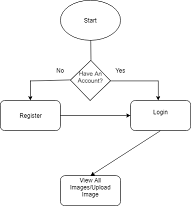
\includegraphics[scale=0.75]{Flow}
\caption{In the following figure is the flow of our system}
\label{fig:flow}
\end{figure}
We tried to simplify the UI as much possible to make the experience more enjoyable, hence the material design.
\begin{figure}[H]
\centering
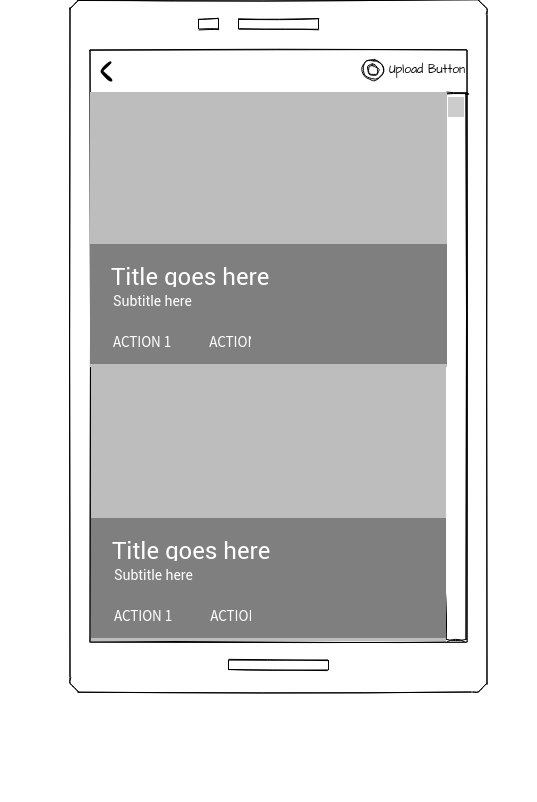
\includegraphics[scale=0.25]{Timeline}
\caption{In the following figure is a wireframe of the user's timeline }
\label{fig:Timeline}
\end{figure}

\subsubsection{Homomorphic Scheme}
We had previously outlined three potential libraries to use for Homomorphic Encryption(HELib,SEAL,PALISADE). We decided to use SEAL as it proved the most beneficial to us.
Since the goal was to use Homomorphic Encryption on a mobile platform which was not natively supported by any library as of the time of writing this, We had to re-compile the SEAL library which was written in C++ and compile it using Java to be compatible with our application.
In general, to run C/C++ code using Java it is done through the Java Native Interface (JNI) which acts as a bridge between Java and C/C++ source file. This process was done as follows, First, we had to use the provided CMake file which is used to manage the building process in a compiler independent manner to import the source files into Android Studio and package them into a library, for this process a lot of errors were encountered due to compatibility issues with different versions of CMAKE.
After managing to port the library into Android Studio the next step was to feed the encrypted data to our neural network however this was not possible as all pre-built Machine Learning libraries and APIs don't support this kind of data so it was necessary to build our neural network from scratch starting from the filters and kernels to the activation functions meaning we would esstentialy have to build our own library which proved to be too challenging and time consuming for this bachelor thesis.

\subsubsection{Data Anonymization}
The main idea in this scheme was to allow the user to choose his own level of privacy by having the user choose his desired social interaction and privacy during the registration process which would affect his experience in the application later on. We defined 3 privacy/social levels for the users to choose from. The levels being,Highest Social Activity and Lowest Privacy,Medium Interaction user and lastly a Non-Social User. Each level then would have certain data anonymization techniques applied to his data.
High Social Users had all their data as it as without any modifications regarding images and text submitted, On the other hand Medium Interaction users had all their image run on a trained face detection machine learning model and applied blurring over resulting faces.These user’s text posts however were posted as it as without any filtering. The model used for facial detection is an *on-device* model and is provided by Google’s firebase ML Kit.
Lastly, the Non-Social users had the most privacy out of the three levels, For images they had the blurring and face detection algorithm run in addition to removing in metadata in images submitted such as location and date.The text posts of these users was also filtered to prevent any locations/names/phone numbers from appearing using a Javascript Natural Language Processing library “Compromise”\cite{Compromise}. We have also added local GUC landmarks and buildings to the lexicon of the library.

PUT IMAGES OF BLURRED FACES AND CENSORED TEXT HERE!

\subsection{Data Obfuscation and de-anonymization}
For this part 2 closely related synthetic datasets where generated. One was designed for friendship inference between students in the GUC and the second one was designed for location inferencing between
students in similar tutorial groups in the GUC.
\subsubsection{Dataset Generation}
Our initial goal was to test whether the Data Obfuscation and de-anonymization experiment localy on students from the GUC however since there was no publicly available dataset we resorted to generating
a synthetic dataset.
Synthetic Dataset generation is commonly used for research purposes as it can be customised to fit the needs of any particular research topic moreover, Institutions and Organizations
have been hesitant to publish any results using any datasets that have been collected from their customers due the recent growing privacy concerns worldwide\cite{dandekar2018comparative}  espically in the EU after 
the latest General Data Proctetion Regulation (GDPR) laws have been passed.
The generated data varies according to the application and research field and may often include text,social connections,images,graphs. The simplest way to generate such datasets is to create
multiple scripts each handling a specific part of the problem the research is tackling and then combine all related rows of data.\cite{albuquerque2011synthetic}\newline
In this paper we chose to use Python to generate our datasets as it has multiple data manipulation libraries namely Numpy and Pandas which are both part of the SciPy package for Python\cite{SciPy}.\newline
For the student friendship prediction dataset we tried to make it as realistic as possible to avoid making it too easy to learn. We tried to model the data that could be generated from 1st year students in a 1 month duration, The design was as follows, each student had a name, 5 intrests chosen randomly out of 20 pre-determined intrests,a tutorial group
that the student is assigned to and finally, each student had a number of "events" that represented his online social presence which could resemble tags in pictures,Facebook mentions,Facebook posts.
To make it more realistic each event had a random number of students participating in it, these students were selected in 2 phases, the first phase was used in the 15 days of the modeling process
where students were selected to be in other student's events randomly which resemble the process that students usually go through when they first join an institution where they are introduced to a large amount of
people as they are seeking to make new friends however as time passes each student's social circle is further reduced to people who are considered friends rather than random people met in lectures, we tried to achieve this
in the final 15 days of the 1 month modeling period by making the participants of the remaining events based on the mutual intrests of students and the number of their previous appearances in the first 15 days of the modeling process.
After generating the data for 150 students we then used cross product to get a record for every student with all the others and finally to decide whether every 2 students should be friends or not, we designed an equation with what we felt
was the most realistic weights for each parameter described above and the final equation was as follows
\begin{equation}
F=0.15(SimilarTutorial)+0.3(MutualIntrests/3)+0.55(MutualEvents^2/15)
\end{equation}
55\% of the weight was given if the number of shared events between the 2 students during the 1 month period was 15 or more events, 30\% of weight was given if the students had atleast 3 mutual intrests
and the last 15\% were given if the students shared the same tutorial. We also considered the values  >0.56 to avoid having un-realistic relations.

\bibliographystyle{acm}
\bibliography{citations}   
\end{document}